\documentclass{article}
\usepackage[utf8]{inputenc}
\usepackage{amsmath}
\usepackage{amssymb}
\usepackage{color}
\usepackage{graphicx}
\usepackage{float}
\usepackage{physics}
\usepackage{caption}
\usepackage{subcaption}
\title{report v0.tex }
\author{Henrik Linder}
\date{\today}
\begin{document}
\maketitle

Given the rates of protein production and decay as 
\begin{equation}
	k_p^{mRNA} = \frac{1}{600}[s^{-1}],\quad k_d = \frac{1}{1800}N_p[s^{-1}],
\end{equation}
we can describe the change in number of proteins $N_p$ as a function of time with the ODE 
\begin{equation}
	\label{eq:protein_ODE}
	\dv {N_p}{t} = k_p^{mRNA}  - k_dN_p .
\end{equation}
By setting $\dv {N_p}{t} = 0 $, we can see that we get a steady state solution when $k_p^{mRNA} = k_dN_p$, or 
\begin{equation}
	\label{eq:steady_state}
	N_p = 3.
\end{equation}


\begin{figure}[H]
	\centering
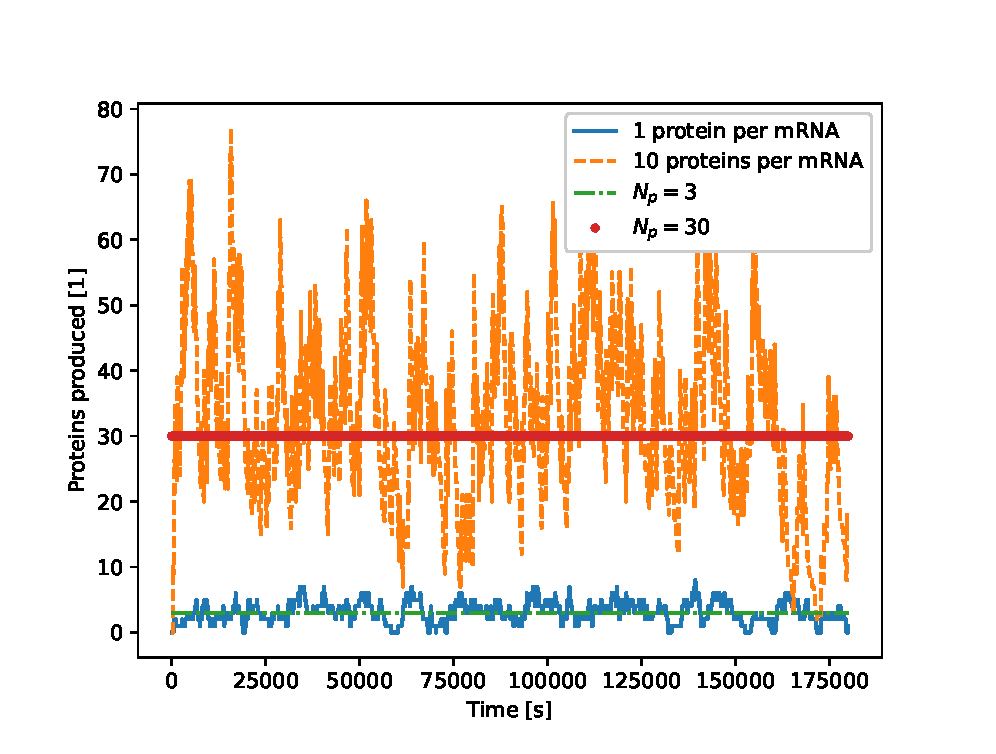
\includegraphics[width = \linewidth]{figs/task1_results_v3.eps}
	\label{fig:task1_results}
	\caption{Protein production versus time for the two simulations in task 1, with 1 and 10 proteins produced per mRNA, respectively. }
\end{figure}
fano 1: 0.8590949869606674, 1.1071931505832386, 0.8251200323666483, 1.1902282676221339
fano 30: 6.156031101748737, 4.70351845831606, 4.887249384566237, 4..031827409953343

After running the simulation ten times, I find that the fano factor ends upbeing about 5 times greater when the mRNA produces 10 proteins than when it produces only one. This seems reasonable since the fano factor is a measure of variation from the mean, and that variation should increase of we increase the size of the random swings. The mean has of course also increased, but the fano factor depends on the square of the variance and only decreases linearly woth the mean, so an oncreased fano factor should come as no surprise. 

\begin{figure}[H]
	\centering
	\begin{subfigure}[b]{.49\textwidth}
		\centering
		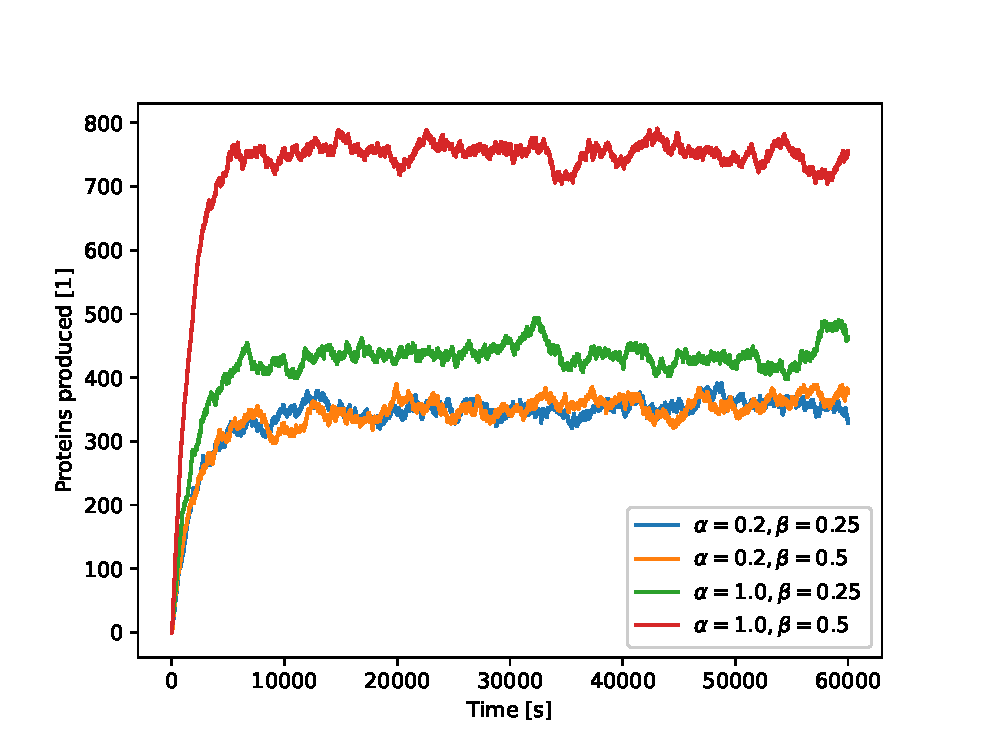
\includegraphics[width = \linewidth]{figs/task2_prot_prod_v4.eps}
		\label{fig:task2_prot_prod}
		\caption{Protein production versus time \\for varying values of $\alpha$ and $\beta$.}
	\end{subfigure}
	\begin{subfigure}[b]{.49\textwidth} 
		\centering
		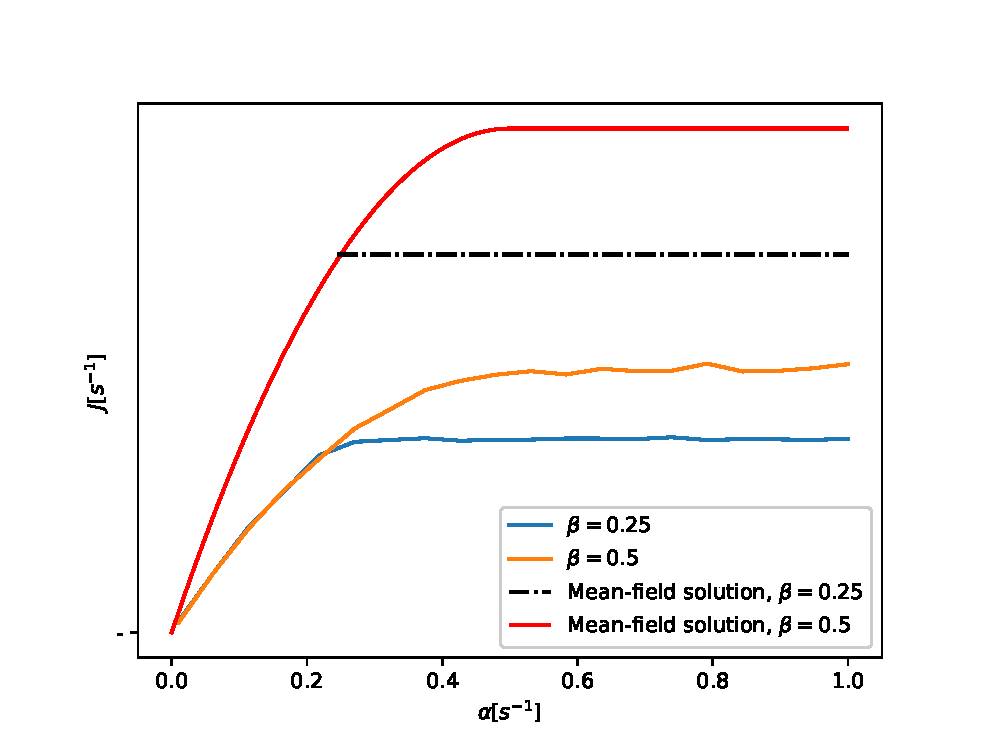
\includegraphics[width = \linewidth]{figs/task2_meanfield_v6.eps}
		\caption{Protein current J plotted against $\alpha$ compared to the mean-field approximation.}
		\label{fig:task2_mean-field}
	\end{subfigure}
	\label{fig:task2}
	\caption{Figures showing the simulated behavior of the protein production and protein current in the simple traffic model of task 2.}
\end{figure}

After running the simulation 10 times, I calculated the Fano factor to be on average 0.73 in this system. That is around the same size as the Fano factor calculated in task 1, indicating that the result is consistent if nothing else. 


fano : [0.599188291198464, 0.72453043417012, 1.2300894353902483, 0.35115527673548463]
mean :  0.72624

As seen in fig.\eqref{fig:task2_mean-field}, the general behavior of my simulation matches the mean-field approximation. However, it differs quite a bit in total number of proteins produced. 
That may be due do the constants used, for example, I am not sure what the translation rate used for the mean-field results were, and it is entirely possible that my translation rate was sub-optimal for the $\alpha$ and $\beta$ used. 

Despite this, I am happy with the results. We can see that the protein current levels off at approximately the same $\alpha$ as the mean-field results for both $\beta$, and the general behavior is the same, showing the linear increase at low $\alpha$ and then leveling off to a constant protein current at higher values of $\alpha$. 

\section{Task3}
fano1 : 1.1537323139033988,  1.0293234725437235, 1.1255733414025437,  0.9870385180083185


fano cont. : 3.4324503269801925, 2.629365078890865, 2.212654090046395, 2.816569373857693

\begin{figure}[H]
	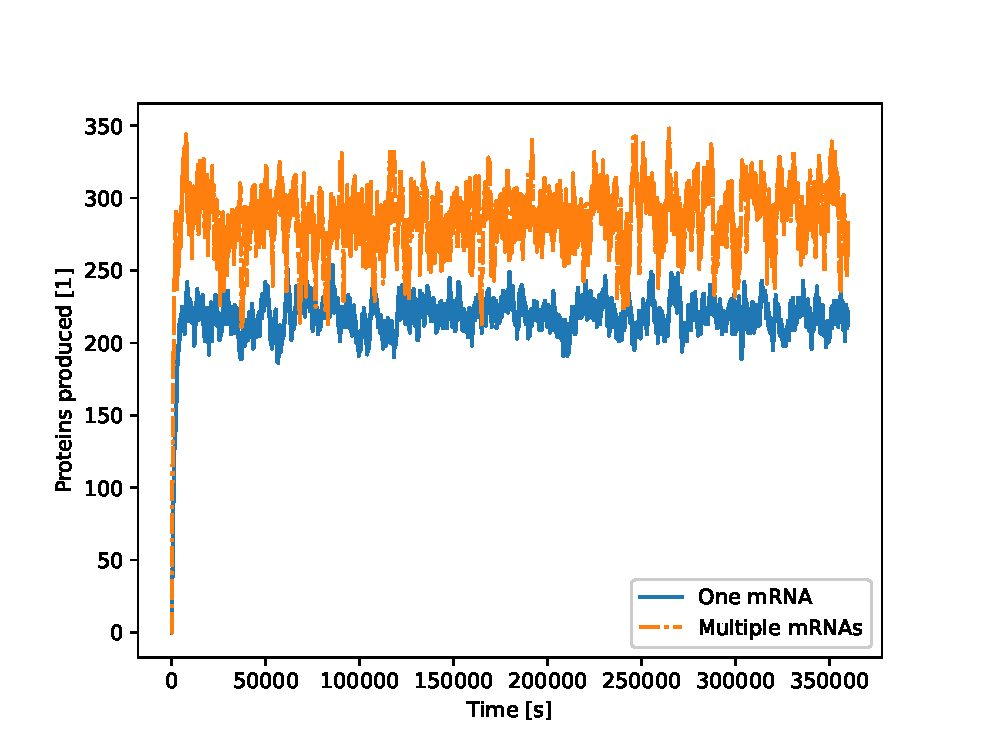
\includegraphics[width=\linewidth]{figs/task3_prot_prod_both_graphs_v2.eps}
	\label{fig:task3}
	\caption{Protein production versus time for both simulations with limited number of ribosomes in task 3. First with only one mRNA, and then with mRNA being created and decaying dynamically. }
\end{figure}

As seen in fig.\eqref{fig:task3}, the protein production is slightly higher with multiple mRNAs than it is with only one. This seems about reasonable since the number of ribosomes has doubled from 4 to 8, increasing the expected protein production. Counteracting this, some of the ribosomes will also be wasted, spending some time on the mRNA before the mRNA decays and releasing the ribosome. I would therefore expect the average number of proteins produced per ribosome to go down. 
%This in not at all surprising since the average number of mRNAs turned out to be slightly below 1 when running my simulation. 

%This may be explained by the fact that the limiting factor is the number of ribosomes. 

The fano factor is much higher in the second case, approximately doubled from 1 to 1.9. This seems fairly reasonable since we are now adding the mechanism of mRNA decay. It is now antirely possible that an mRNA will be produced, exist for a while, then decay without ever producing a protein. It will however keep ribosomes busy, only releasing them into the free pool upen decay. This may all explain the increased burstiness of the system. 





\section{Task4}
The discrepancy between this model and the real-world behavior of the protein production may be caused by any of a number of factors, but the one that comes to mind is transcription factors (TFs). These affect the transcripton of DNA into mRNA. They react to external signals and bind to the DNA, activating or repressing the transcription of a certain gene

Another mechanism for regulating the protein production is Small RNA regulation. This is where small pieces of RNA attach to the mRNA, blocking the ribosome from passing, effectively stopping the translation of that piece of mRNA. 

Neither of these mechanisms are caught in our model, indicating that we won't be able to reach a realistic real-world behavior for the protein production without modifications. 

\begin{figure}[H]
	\centering
	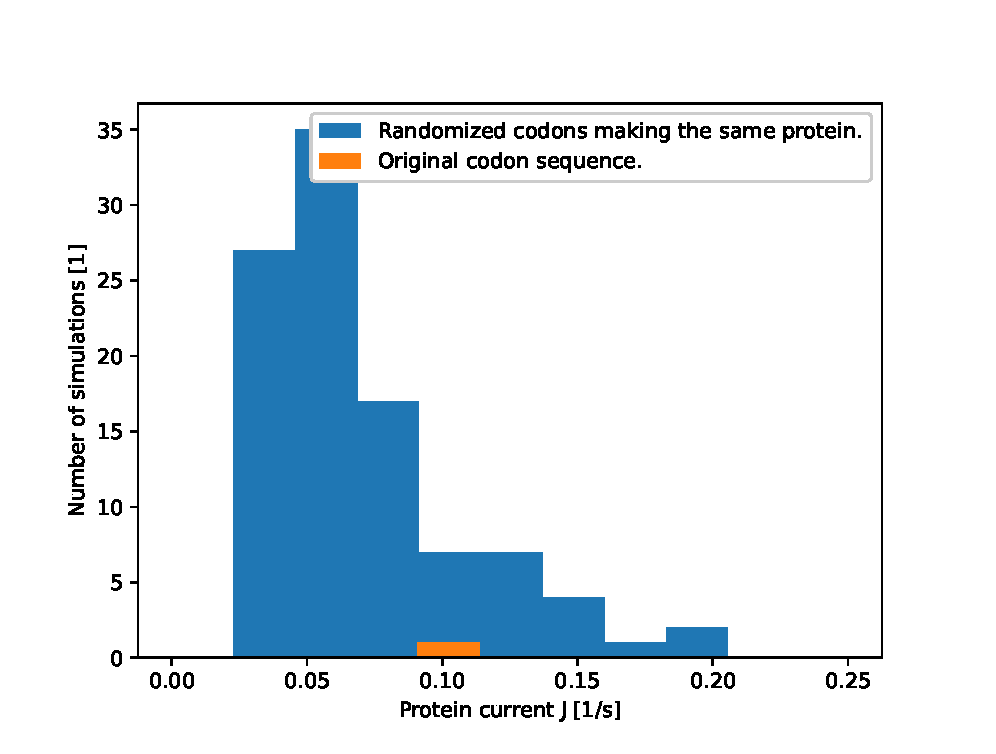
\includegraphics[width=\linewidth]{figs/task4_histogram_labversion_v0.eps}
	\label{fig:task4_histogram}
\end{figure}

\begin{figure}[H]
	\centering
	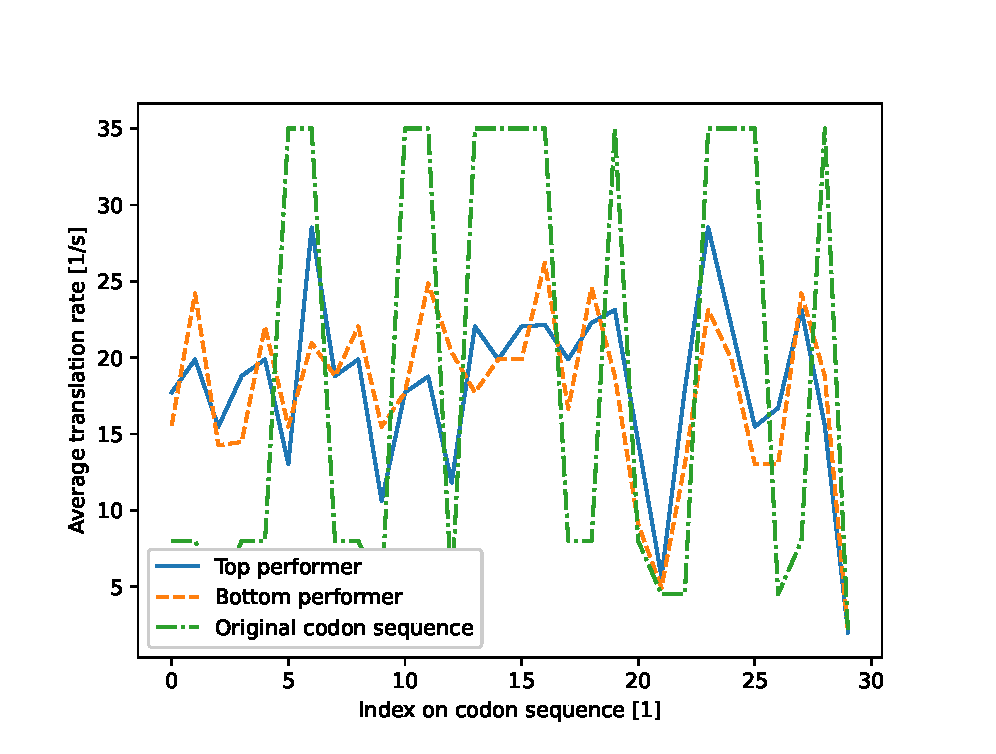
\includegraphics[width=\linewidth]{figs/task4_rateplot_labversion_v0.eps}
	\label{fig:task4_rateplot}
\end{figure}

\begin{figure}[H]
	\centering
	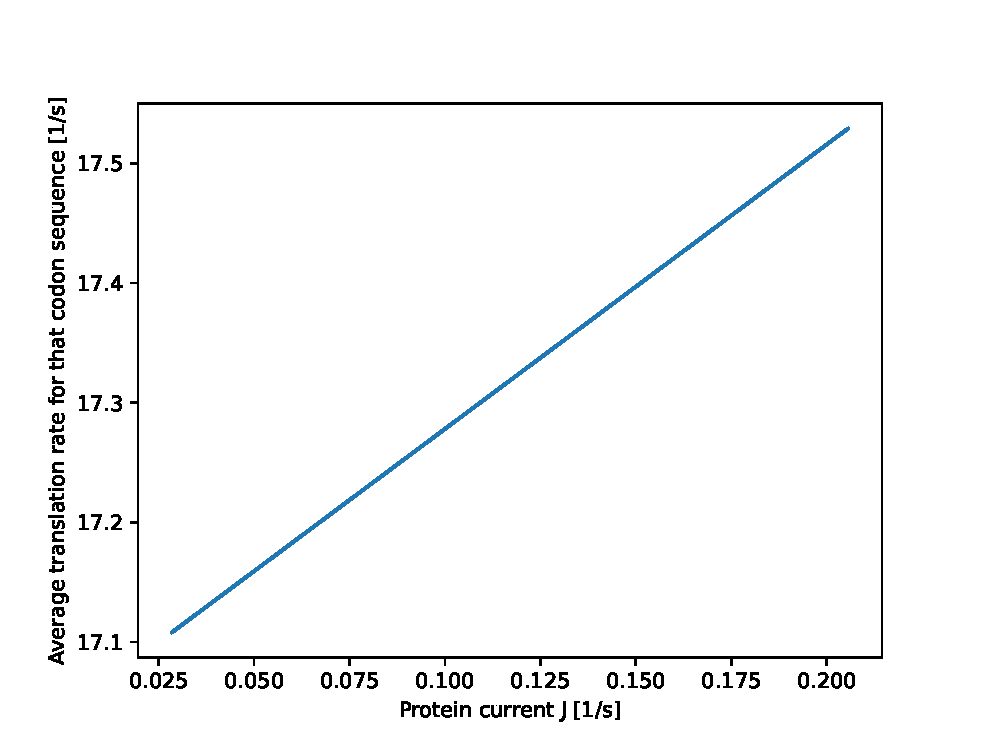
\includegraphics[width=\linewidth]{figs/task4_linfit_labversion_v0.eps}
	\label{fig:task4_linfit}
\end{figure}
As shown in figure \eqref{fig:task4_linfit}, if we do a linear fit between the Protein current $J$ and the average translation speed $q$ for the correnspinding codon sequence, we see that there is a slight positive correlation. It should come as no surpise that a higer average translation speed corresponds to a higher protein current, but it is still nice to have it confirmed. 


As we can observe in figure  \eqref{fig:task4_rateplot}, there is a marked difference in the behavior of the original codon sequence as compared to that of the other ones shown. I have a sneaking suspicion that this is because this sequence was chosen for its staggered translation rate, as it is very appropriate for this lab. Either that or it is just a happy coincidence. 
Either way, as a result of the averaging process, both the top and bottom performers are closer to the middle, with more even translation rates. However, the 


Average rates for top performers: 
 [20.69354839]
 [18.19354839]
 [21.90322581]
 [18.08064516]
 [18.30645161]

Average rates for bottom performers: 
[17.5483871 ]
 [17.20967742]
 [13.61290323]
 [17.32258065]
 [19.06451613]

\end{document}
